In der Optik geht man von Licht als Welle aus. Genauer gesagt wird Licht als elektromagnetische Welle betrachtet. Ein Gegensatz dazu wäre die Betrachtung von Lichtquanten, auch Lichtteilchen oder Photonen genannt. (Siehe \referenz{sec:lichtteilchenwelle} für eine Gegenüberstellung.)

Als elektromagnetische Wellen bezeichnet man alle Wellen, bei denen gekoppelte elektrische und magnetische Felder schwingen. Die Schwingungsverktoren der beiden Felder stehen jeweils senkrecht aufeinander und senkrecht auf dem Vektor der Ausbreitungsrichtung:\endnote{„Onde electromagnetique“ von SuperManu - Self, based on Image:Onde electromagnetique.png. Lizenziert unter CC BY-SA 3.0 über Wikimedia Commons - \url{https://commons.wikimedia.org/wiki/File:Onde_electromagnetique.svg}}

\begin{figure}[h!]
	\center
	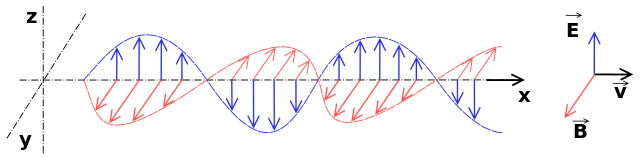
\includegraphics[width=0.8\textwidth]{em_welle}
	\caption{Eine elektromagnetische Welle}
	\label{fig:emwelle}
\end{figure}

Im Vakuum, beziehungsweise in der Luft, bewegen sich alle elektromagnetischen Wellen mit einer konstanten Geschwindigkeit fort, der Vakuumlichtgeschwindigkeit. (\casio{28}: $c_0=299.792.458 \frac{m}{s}$)

\subsection{Spektrum}

\hspace{-17pt}
\begin{tabular}[c]{|c|c|c|l|}
	\hline
	Name				&	$f$						& $\lambda$ 	& Kommentar\\
	\hline
	Längstwellen		&	$15-200Hz$				& $10^6-10^7m$ & Strom; Nur Nahfeld\\
	Radiowellen			&	$10^4-10^8Hz$			& $10^0-10^4m$ & \\
	Mikrowellen			&	$10^8-10^{11}Hz$		& $10^{-3}-10^{0}m$ & \\
	Infrarotes Licht	&	$>10^{12}Hz$			& $<10^{-4}m$ & \glqq Wärmestrahlung\grqq \\
	Sichtbares Licht	&	$\approx 10^{15}Hz$		& $400-800nm$ & sichtbar\\
	Röntgenstrahlung	&	$10^{16} - 10^{20}Hz$	& $10^{-12}-10^{-8}m$ & Erzeugung: $e^{-}$ auf Metall \\
	Gammastrahlung		&	$>10^{20}Hz$			& $<10^{-12}m$ & \\
	\hline
\end{tabular}
